Para efectuar el calculo directo de la DFT haciendo uso de la herramienta MATLAB se implementa la función \texttt{X= DFTsum(x)} para obtener la DFT de N puntos, siendo \texttt{x} el parámetro corresponde a una señal de entrada \textit{x(n)} la cual desarrolla la ecuación \ref{DFT} en base a \textit{ciclos-for} calculando a la vez los exponenciales directamente. Esta código de implementación de la función se presenta a continuación

\begin{lstlisting}[language = octave]
function X = DFTsum(x)
    N = length(x);
    X = zeros(1,N);
    for k = 0:N-1
        coef = exp(-1j*2*pi*k/N);
        for n = 0:N-1
            X(1,k+1) = X(1,k+1) + x(n+1)*coef^n;
          
        end
        
    end
    
end
\end{lstlisting}


\begin{equation}
    X_N(k) = X^{(N)}(k) = \sum_{n = 0}^{N-1} x(n)e^{-j2\pi k n /N}
    \label{DFT}
\end{equation}

\begin{enumerate}
    \item Para probar la función implementada se generaron las siguientes señales 
    
    $$ x_1(n) = \delta (n)$$
    $$ x_2(n) = 1$$
    $$ x_3(n) =e^{-j2 \pi n /N}$$
    $$ x_4(n) = cos(2\pi n /N)$$
    
    
    Se grafica la salida de la función en el rango $[-\pi, \pi]$ para cada señal considerando 8 muestras para cada una, se  grafica además, en el mismo rango de valores el resultado que entrega MATLAB al aplicar el comando \texttt{fft} a las señales generadas. Las gráficas mencionadas se muestran en la figura \ref{DFTsum}
    
    \begin{figure}[H]
        \centering
        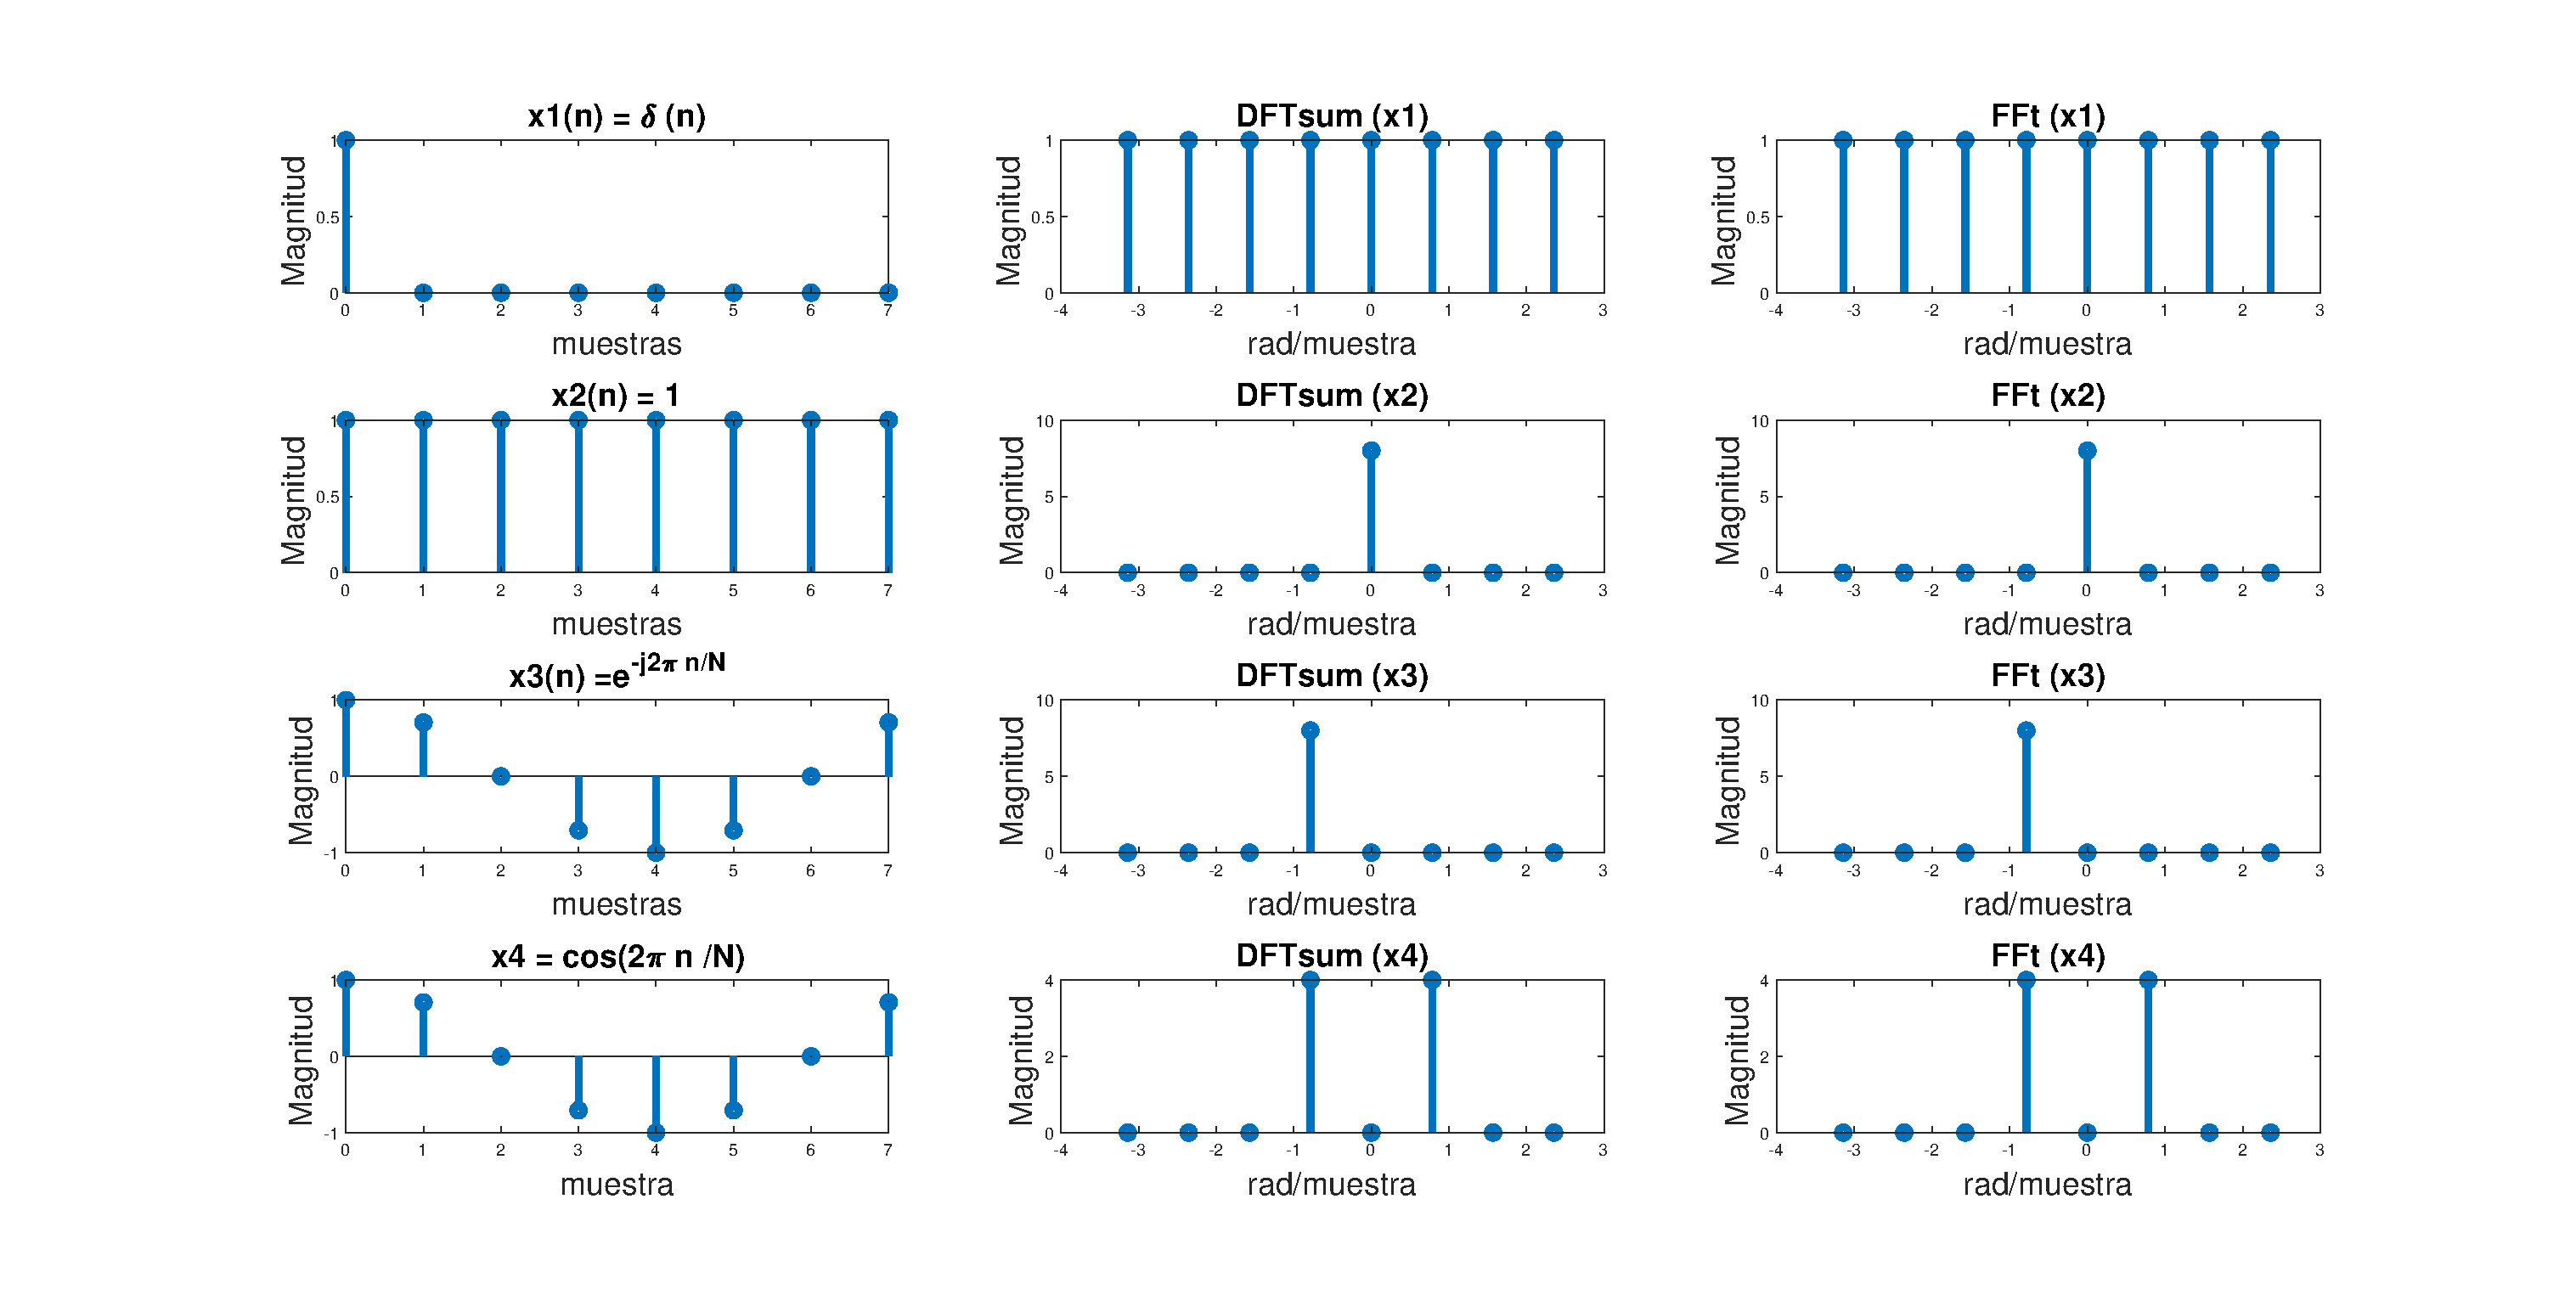
\includegraphics[scale = 0.3]{Figuras/p4_1-DFTsum.eps}
        \caption{Señales $x_1$, $x_2$, $x_3$ y $x_4$ generadas junto a sus respectivas DFT obtenida con la función implementada y FFT obtenida con comandos en MATLAB}
        \label{DFTsum}
    \end{figure}


Se puede apreciar cómo el resultado que se obtiene mediante el comando \texttt{fft} de MATLAB es idéntico al que se obtiene al utilizar la función \texttt{DFTsum} siendo consistente con lo que se espera de su funcionamiento según la teoría. En el caso particular de la señal $x_3$ que corresponde a una señal compleja se presenta  gráfica solo de la parte real asociada a su espectro en frecuencia por lo que el resultado es similar al de la señal $x_4$ pero con un solo impulso (\textit{recordar $2cos(\phi) = e^{j\phi} + e^{j\phi}$}).


Usando el comando de MATLAB \texttt{immse} se obtuvo la siguiente tabla resumen entre los valores numéricos obternidos usando la función \texttt{DFTsum} y el resultado entregado por el comando \texttt{fft} de MATLAB


 \begin{table}[H]
        \centering
        \begin{tabular}{|c|c|}
        \hline
         Señal    & MSE $DFT~~ v/s~~ fft$  \\
         \hline
         $x_1(n) = \delta (n)$   & $0$ \\
         \hline
          $x_2(n) = 1$   &   $1.2195\cdot 10^{-30}$ \\
         \hline
            $ x_3(n) =e^{-j2 \pi n /N}$ &   $7.1631\cdot 10^{-31} $\\
         \hline
        
         $ x_4(n) = cos(2\pi n /N)$  &    $3.1880\cdot 10{-31}  $\\
         \hline


        \end{tabular}
        \caption{Cuadro resumen para el error cuadrático medio entre el resultado de la función \texttt{DFTsum} y el resultado entregado por el comando \texttt{fft} de MATLAB para cada señal de prueba.}
        \label{MSE}
    \end{table}
    
    %4.2
    \item
    
    
    %4.3
    \item Se considera la señal $x_1(t) = cos(wt)$ con frecuencia de 100 Hz, muestreada a 5kHz durante 1000 ms. 
    
    Se grafica el error en la magnitud del espectro obtenido con la función \texttt{DFTsum} y \texttt{fft}. Dicho gráfico se muestra en la figura \ref{fig:p4_3err}, donde se observa un máximo error del orden de $10^{-9}$, por lo que se asume despreciable. El error cuadrático medio obtenido es de $5.4744 \cdot 10^{-22}$.
    
    \begin{figure}[H]
        \centering
        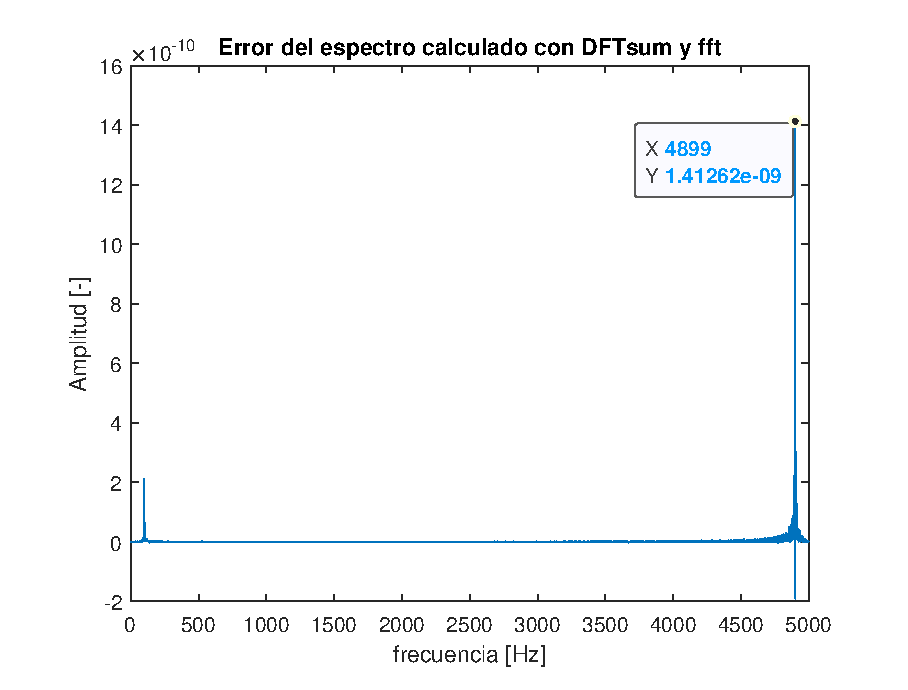
\includegraphics[width = 0.8\linewidth]{Figuras/p4_3err.eps}
        \caption{Error de magnitud del espectro utilizando \texttt{DFTsum} con respecto a \texttt{fft} en MATLAB.}
        \label{fig:p4_3err}
    \end{figure}
     
     

    

    
\end{enumerate}

